\documentclass[residuals.tex]{subfiles}

\begin{document}


\section{Assumption of Constant Variance}
\subsection*{Homoscedasticity}
\begin{itemize}
*  \textbf{\textit{Homoscedascity}} is the technical term to describe the variance of the residuals being constant across the range of predicted values. 

*  \textbf{\textit{Heteroscedascity}} is the converse scenario : the variance differs along the range of values.
\end{itemize}


\noindent Suppose you plot the individual residuals against the predicted value, the variance of the residuals predicted value should be constant. 
\bigskip
\noindent Consider the red arrows in the picture below, intended to indicate the variance of the residuals at that part of the number line. For the OLS summption to be valid , the length of the red lines should be more or less the same.


\begin{framed}

\begin{verbatim}	



# Evaluate homoscedasticity

# non-constant error variance test

library(car)
ncvTest(fit)
\end{verbatim}
\end{framed}


\begin{figure}[h!]
\centering
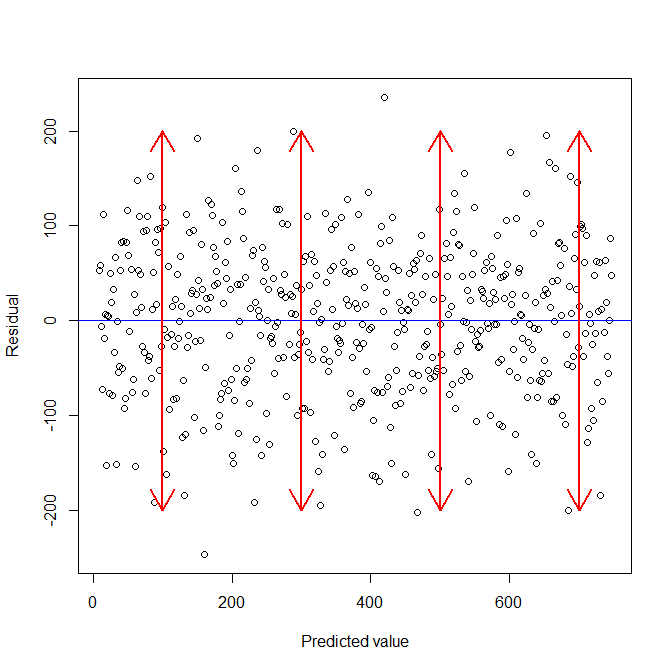
\includegraphics[width=0.6\linewidth]{homosked}
\caption{}
\label{fig:homosked}
\end{figure}



\begin{figure}[h!]
\centering
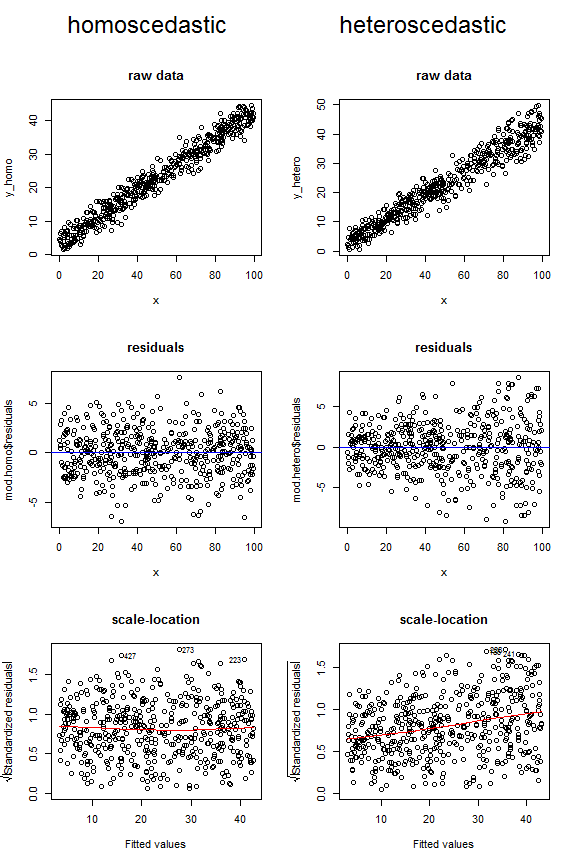
\includegraphics[width=0.7\linewidth]{homosked2.png}
\caption{}
\label{fig:homosked2}
\end{figure}


%================================================================= %

\subsection{Nonlinearity}

\begin{framed}

\begin{verbatim}	
	

# Evaluate Nonlinearity

# component + residual plot 


crPlots(fit)


# Ceres plots 

ceresPlots(fit)


Non-independence of Errors
# 
Test for Autocorrelated Errors

durbinWatsonTest(fit)

\end{verbatim}

\end{framed}

%http://stats.stackexchange.com/questions/58141/interpreting-plot-lm
%\texttt{I explained the assumption of homoscedasticity and the plots that can help you assess it (including scale-location plots [2]) on CV here: What does having constant variance in a linear regression model mean? I have discussed qq-plots [3] on CV here: QQ plot does not match histogram. So, what's left is primarily just understanding [5], the residual-leverage plot.}
In a multiple linear regression, it is assumed that the dependence on each of the predictors is linear. The partial residual plot has been available as a diagnostic, but it can fail if there are nonlinear relationships among the predictors. The Mallows augmented partial residual plot is effective even if there are quadratic relationships among the predictors. Dennis Cook developed the CERES plot to show a curve in the relationship of the dependent variable to a predictor, in spite of any nonlinear relationships among the predictors.
\end{document}
